\documentclass{beamer}
\usetheme{metropolis}
\usepackage{graphicx}
\usepackage{subfig}
\usepackage{hyperref}
\usepackage{tcolorbox}
\title{Calculus-Based Physics-1: Mechanics (PHYS150-01): Week 7}
\date{October 16th - October 20th, 2017}
\author{Jordan Hanson}
\institute{Whittier College Department of Physics and Astronomy}

\begin{document}
\maketitle

\section{Week 6 Review}

\begin{frame}{Week 6 Review}
\begin{enumerate}
\item \alert{Work} has a scientifically precise definition
\begin{itemize}
\item Units
\item As a product of force and displacement vectors
\end{itemize}
\item Kinetic Energy and the \alert{Work-Energy Theorem}
\item Gravitational potential energy
\begin{itemize}
\item Potential energy
\item \textit{Simplifying otherwise complex calculations}
\item Potential energy near Earth's surface
\item ...in space
\end{itemize}
\item Definition of a \textbf{conservative force}
\begin{itemize}
\item Relationship between conservative forces and potential energy
\item Conservation of energy for conservative forces
\end{itemize}
\end{enumerate}
\end{frame}

\section{Week 6 Review Problems}

\begin{frame}{Week 6 Review Problem}
Recall that the \textit{gravitational potential energy} associated with an object of mass $m$ located a height $y$ above ground level is $U = mgy$.  What is $-dU/dy$?
\begin{itemize}
\item A: $mg$
\item B: $-mg$
\item C: $g$
\item D: $-g$
\end{itemize}
\end{frame}

\begin{frame}{Week 6 Review Problem}
What is the physical meaning of the quantity $-mg =-dU/dy$?
\begin{itemize}
\item A: The force of gravity 
\item B: The acceleration due to gravity
\item C: The mass
\item D: Change in kinetic energy
\end{itemize}
\end{frame}

\section{Week 7 Summary}

\begin{frame}{Week 6 Summary}
\begin{enumerate}
\item \alert{Work} and \alert{potential energy}
\begin{itemize}
\item \textbf{Lab activity:} Oscillator and gravity trading work and potential energy
\end{itemize}
\item Potential energy and \textbf{conservative forces}
\item \alert{\textbf{Conservation of Energy}}
\begin{itemize}
\item \textit{Calculus review: the fundamental theorem of calculus}
\item Graphical representations of integrals and energy
\end{itemize}
\end{enumerate}
\end{frame}

\section{Work and Potential Energy}

\begin{frame}{Work and potential energy}
When we do work on a system, even if in the final state the system has no velocity, it can still have energy.  The concept of \textit{potential energy} is \textbf{like thinking of work backwards}:
\begin{itemize}
\item If we compress an oscillator (a spring), and keep compressing it, it has no kinetic energy but it will have kinetic energy if we release it.
\item If we raise an object against the force of gravity to a certain height, it has no kinetic energy but it will have kinetic energy if we drop it.
\item \alert{But it took work to create this change in kinetic energy, from the work-energy theorem.} 
\end{itemize}
\textit{Systems are not necessarily \textbf{required} to operate like this...Think of stretching plastic or dough.  Where does the work go?}
\end{frame}

\begin{frame}{Work and potential energy}
The relationship between work and potential energy therefore resembles (by definition) the opposite of the work-energy theorem:
\begin{equation}
\Delta U_{\rm AB} = U_{\rm B} - U_{\rm A} = -W_{\rm AB}
\end{equation}
\end{frame}

\begin{frame}{Work and potential energy}
\begin{figure}
\centering
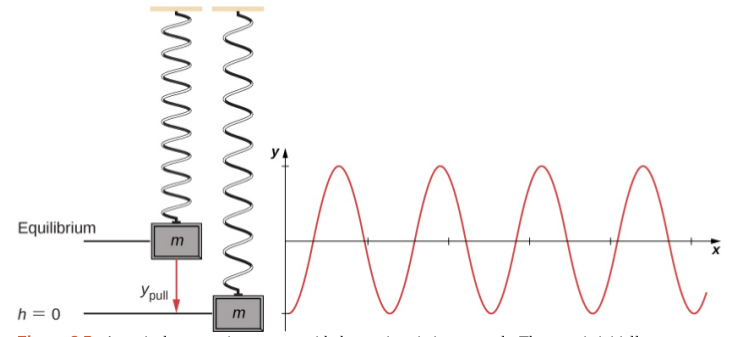
\includegraphics[width=0.9\textwidth,trim=0cm 0.1cm 0cm 0cm,clip=true]{figures/osc.png}
\caption{\label{fig:osc} An oscillator is stretched to a new equilibrium point by gravity.  When pulled a certain distance down, or compressed a certain distance upwards, $y_{\rm pull}$, we observe oscillation.}
\end{figure}
\end{frame}

\begin{frame}{Work and potential energy}
\begin{figure}
\centering
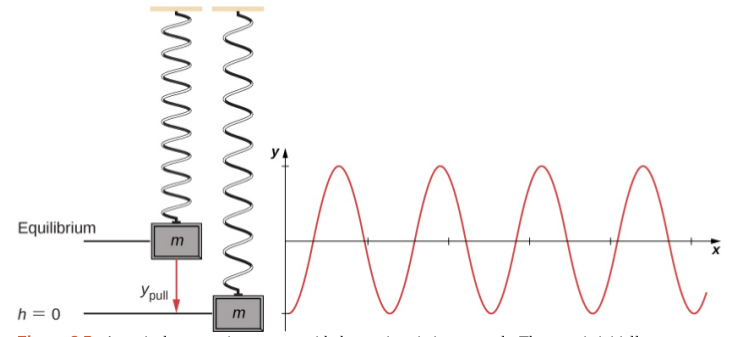
\includegraphics[width=0.9\textwidth,trim=0cm 0.1cm 0cm 0cm,clip=true]{figures/osc.png}
\caption{\label{fig:osc2} Notice that it does not matter what the observer defines as \textit{zero} potential energy, since work is required to perform \textit{changes} in potential energy.}
\end{figure}
\end{frame}

\begin{frame}{Work and potential energy}
\begin{figure}
\centering
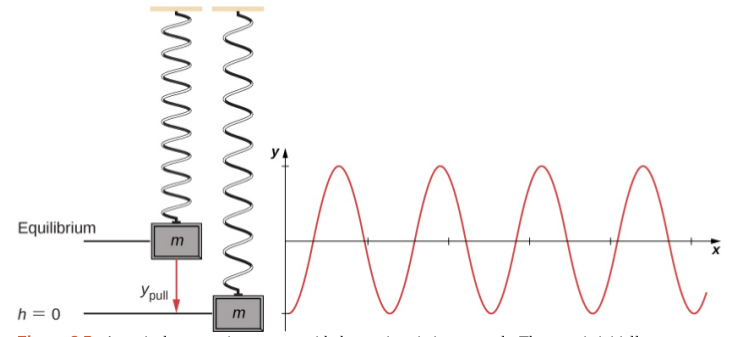
\includegraphics[width=0.9\textwidth,trim=0cm 0.1cm 0cm 0cm,clip=true]{figures/osc.png}
\caption{\label{fig:osc3} The fact that work is required only to perform changes in potential energy, but not does not determine the \textit{absolute scale} of potential energy, means the observer \alert{may choose the location of zero potential energy}, in the same fashion as choosing a coordinate system.}
\end{figure}
\end{frame}

\begin{frame}{Work and potential energy}
\begin{figure}
\centering
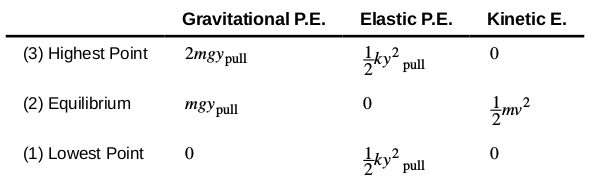
\includegraphics[width=0.9\textwidth,trim=0cm 0.1cm 0cm 0cm,clip=true]{figures/table.png}
\caption{\label{fig:osc4} If a mass $m$ is connected to the oscillator and \textit{we choose} the potential energy zero-point to be \textbf{the low point of oscillation}, the values listed in this table correspond to the energies at various states.}
\end{figure}
\end{frame}

\section{Lab Activity - Gravity and the Oscillator}

\begin{frame}{Lab Activity: Work and Potential Energy}
\small
\begin{itemize}
\item Using the springs, weights, hooks, and system of clamps and grips, build a vertical oscillating system.
\item Diagram the system, showing a clearly defined value for $y_{\rm pull}$, and a clearly defined choice for the potential energy zero-point.
\item Measure the \textit{unstretched} spring length, and the \textit{equilibrium length} caused by gravity, to \textbf{derive the spring constant $k$}.  Quote the value of $k$ in N/m.
\item Pull the spring downwards by $y_{\rm pull}$, and record the maximum and minimum heights of the weight as the spring oscillates it.
\item Create a table like Tab. \ref{fig:osc4}, and fill in the actual energy values in Joules.  What is your predicted value for $v$, the speed at which the weight moves when the oscillator is at the equilibrium position?
\end{itemize}
\end{frame}

\begin{frame}{Work and potential energy}
\begin{figure}
\centering
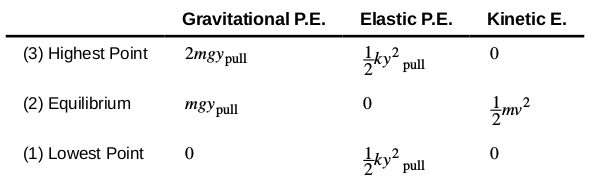
\includegraphics[width=0.9\textwidth,trim=0cm 0.1cm 0cm 0cm,clip=true]{figures/table.png}
\caption{\label{fig:osc5} If a mass $m$ is connected to the oscillator and \textit{we choose} the potential energy zero-point to be \textbf{the low point of oscillation}, the values listed in this table correspond to the energies at various states.}
\end{figure}
\end{frame}

\section{Lab Activity - Gravity and the Oscillator, Part 2}

\begin{frame}{Lab Activity: Work and Potential Energy}
\small
\begin{itemize}
\item Measure the \textit{unstretched} spring length, and the \textit{equilibrium length} caused by gravity, to \textbf{derive the spring constant $k$}.  Quote the value of $k$ in N/m.
\item Pull the spring downwards by $y_{\rm pull}$, and record the maximum and minimum heights of the weight.
\item Create a table like Tab. \ref{fig:osc4}, and fill in the actual energy values in Joules.  What is your predicted value for $v$?
\item Using the \textbf{Vernier LabPro} and the \textit{motion detector attachment}, measure $v$ when the spring is at equilibrium position, and quote the value in m/s.  Does it agree with your prediction based on energy conservation?  Why or why not?
\end{itemize}
\end{frame}

\begin{frame}{Work and potential energy}
\begin{figure}
\centering
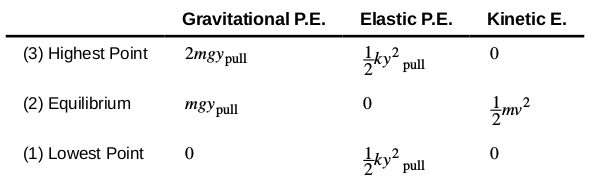
\includegraphics[width=0.9\textwidth,trim=0cm 0.1cm 0cm 0cm,clip=true]{figures/table.png}
\caption{\label{fig:osc6} The value for $v$ is predicted by energy conservation.  What do you measure?}
\end{figure}
\end{frame}

\section{Potential Energy and Conservative Forces}

\begin{frame}{Potential Energy and Conservative Forces}
Let path 1 be be through a force field that does work $W_{\rm 1}$ on a system, and path 2 be a different path that does work $W_{\rm 2}$ on a system.
\begin{equation}
W_{\rm 1} = \int_{\rm Path 1} \vec{F}\cdot d\vec{r} = \int_{\rm Path 2} \vec{F} \cdot d\vec{r} = W_{\rm 2}
\end{equation}
A force is conservative if 
\begin{equation}
W_{\rm 1} = W_{\rm 2}
\end{equation}
Suppose path 1 goes from point A to B, and path 2 returns from B to A.  If the force remains constant, but the path is reversed, then $W_{\rm 1} = -W_{\rm 2}$.  But this means the path is \textit{closed}, so 
\begin{equation}
\oint \vec{F} \cdot d\vec{r} = W_{\rm 1} + W_{\rm 2} = W_{\rm 1} - W_{\rm 1} = 0
\end{equation}
\end{frame}

\begin{frame}{Potential Energy and Conservative Forces}
How do you show that a force is conservative?  We cannot test \textbf{all possible paths}.  This is a question for \textit{vector calculus}.  The results are straightforward to memorize:
\begin{equation}

\end{equation}
\end{frame}

\section{Conclusion}

\section{Answers}

\begin{frame}{Answers}
\begin{columns}[T]
\begin{column}{0.5\textwidth}
\begin{itemize}
\item $-mg$
\item The force of gravity 
\end{itemize}
\end{column}
\begin{column}{0.5\textwidth}
\begin{itemize}
\item ...
\end{itemize}
\end{column}
\end{columns}
\end{frame}

\end{document}
